% !TEX root = main.tex
\section{システム構成}
\subsection{システム全体図}
本研究で構築したシステムの全体図を図\ref{fig:system_diagram}に示す.
本システムは,下位レイヤーと上位レイヤーの2つの主要な構成要素からなる.

\begin{figure}[h]
    \centering
    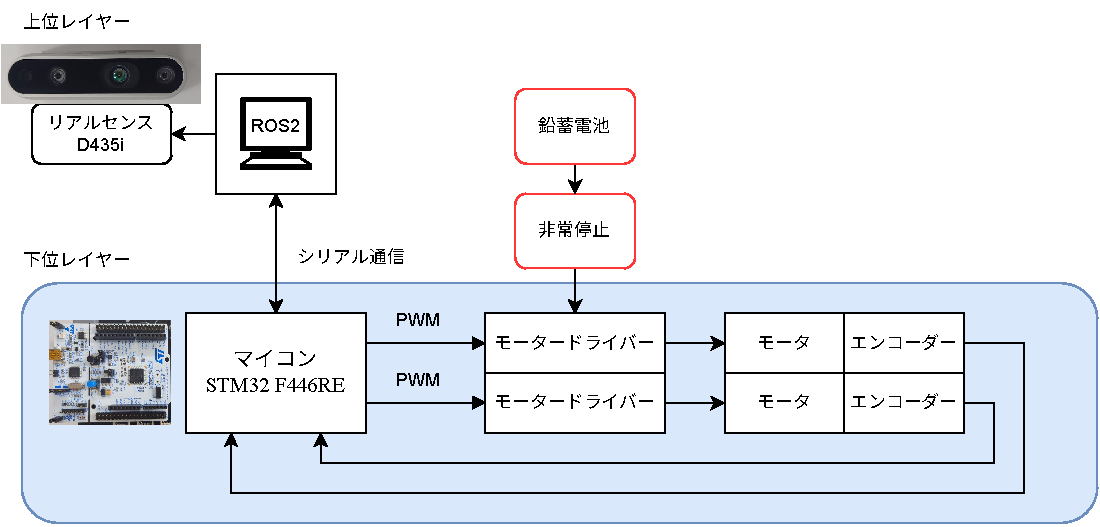
\includegraphics[width=1.0\textwidth]{figure/system.pdf}
    \caption{システム全体図}
    \label{fig:system_diagram}
\end{figure}

% === ハードウェア ==========================================================

\subsection{ハードウェア構成}
本システムのハードウェア構成について,以下に各要素を説明する.

\subsubsection{マイコン(STM32 Nucleo Board STM32F446RE)}
本システムでは,STM32 Nucleo Board STM32F446REマイコンボードを使用している.
STM32 F446REは高性能なARM Cortex-M4プロセッサを搭載しており,以下の特徴を持つ.
\begin{itemize}
    \item 最大180 MHzのクロック速度
    \item タイマーをエンコーダモードに設定可能
    \item 開発/評価ボードであり入手性が高い
\end{itemize}
本マイコンは,モーター駆動,エンコーダーのデータ取得を担当しており,
ロボットの下位制御レイヤーを実現している.


\subsubsection{エンコーダー(AMT102-V)}
AMT102-Vエンコーダーを採用し,モーターの回転角速度および回転位置を計測している.
図\ref{fig:AMT102}に使用するエンコーダーを示す.
このエンコーダーは最大分解能は2048 PPR(Pulse Per Revolution)であり,
非接触方式である.
エンコーダーからの信号はマイコンで処理され,
車輪の速度制御や自己位置推定に使用する.

\begin{figure}[H]
    \centering
    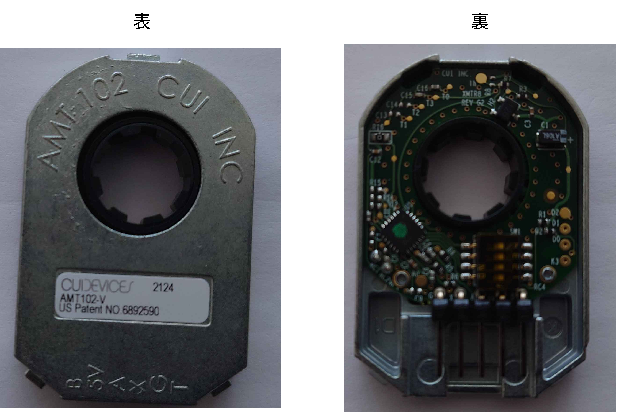
\includegraphics[width=0.5\textwidth]{figure/AMT102.pdf}
    \caption{AMT102-V}
    \label{fig:AMT102}
\end{figure}

\subsubsection{深度カメラ(Intel RealSense D435i)}
深度カメラとしてIntel RealSense D435iを採用している.D435iは,ステレオカメラ方式に基づく高精度な距離計測を特徴とし,以下のような仕様を持つ.
\begin{itemize}
    \item 最大測定距離:0.1~10メートル
    \item フレームレート:最大90 FPS
    \item 視野角:水平87°,垂直58°
    \item IMU(慣性計測ユニット)搭載
\end{itemize}
本システムでは,D435iから取得した深度データを用いて目標(人)の位置を検出し,
追従アルゴリズムに利用している.

\begin{figure}[H]
    \centering
    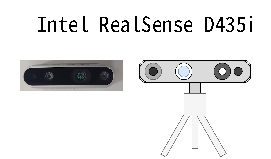
\includegraphics[width=0.5\textwidth]{figure/RealSense.pdf}
    \caption{AMT102-V}
    \label{fig:RealSense}
\end{figure}


% === ソフトウェア ==========================================================
\subsection{ソフトウェア構成}
本システムのソフトウェア構成について,以下に各要素を説明する.

\subsubsection{下位レイヤー}
本システムの下位レイヤーソフトウェアでは,モーター制御,エンコーダーのデータ処理,
およびシリアル通信を実現するために自作ライブラリを使用している.
以下に,各ライブラリの詳細について説明する.

\paragraph{エンコーダーライブラリ (encoder.c, encoder.h)}
エンコーダーライブラリは,ロータリーエンコーダー(AMT102-V)の値を取得し,
角速度や回転数を計算するための機能をもつ.
このライブラリでは,エンコーダーから得られる値を高精度に利用するために4逓倍処理を行い,
モーターの速度制御に使用している.以下に,一部ライブラリコードを示す.

\lstset{language=C}
\begin{figure}[H]
    \centering
    \begin{lstlisting}
int Encoder_Read(Encoder* encoder)
{
    int16_t count = (int16_t)(__HAL_TIM_GET_COUNTER(encoder->htim) - TIMER_MAX_COUNT / 2);
    return count;
}
        
void Encoder_Interrupt(Encoder* encoder, EncoderData* encoder_data)
{
    int count = Encoder_Read(encoder);
        
    encoder_data->count = count;
    encoder_data->rot = count / (double)encoder->ppr;
    encoder_data->deg = encoder_data->rot * 360.0;
    encoder_data->distance = encoder_data->rot * (PI * encoder->diameter);
        
    encoder_data->rps = (encoder_data->rot - encoder->before_rot) / (encoder->period * 0.001);
    encoder_data->velocity = encoder_data->rps * PI * encoder->diameter;
        
    encoder->before_rot = encoder_data->rot;
}
    \end{lstlisting}
    \caption{エンコーダーカウント値の取得 (encoder.c)}
    \label{lst:encoder_count}
\end{figure}

また,このライブラリではカウント値のリセット機能も提供しており,
特定の条件下でカウント値をゼロに戻すことが可能である.

\paragraph{モータードライバライブラリ (motor\_driver.c, motor\_driver.h)}
モータードライバライブラリは,DCモーターの速度と方向を制御するための機能をもつ.
このライブラリでは,PWM信号を用いてモーターを駆動し,
回転方向の切り替えや速度制御を行っていおる.以下に,一部ライブラリコードを示す.

\begin{figure}[H]
    \centering
    \begin{lstlisting}
// 初期化関数
void MotorDriver_Init(MotorDriver* motor, TIM_HandleTypeDef* htimA, uint32_t channelA,TIM_HandleTypeDef* htimB, uint32_t channelB) {
motor->htimA = htimA;
motor->channelA = channelA;
motor->htimB = htimB;
motor->channelB = channelB;    
 // PWM開始
HAL_TIM_PWM_Start(htimA, channelA);
HAL_TIM_PWM_Start(htimB, channelB);
}
// 速度設定関数
void MotorDriver_setSpeed(MotorDriver *motor, int speed) {
    int pwm_value;
    if (speed > 100) speed = 99;     //ブーストラップ回路に対応
    if (speed < -100) speed = -99;   //ブーストラップ回路に対応
        
    if (speed > 0) {
        pwm_value = (speed * __HAL_TIM_GET_AUTORELOAD(motor->htimA)) / 100;
        __HAL_TIM_SET_COMPARE(motor->htimA, motor->channelA, pwm_value);
        __HAL_TIM_SET_COMPARE(motor->htimB, motor->channelB, 0);
    } else {
        pwm_value = (-speed * __HAL_TIM_GET_AUTORELOAD(motor->htimA)) / 100;
        __HAL_TIM_SET_COMPARE(motor->htimA, motor->channelA, 0);
        __HAL_TIM_SET_COMPARE(motor->htimB, motor->channelB, pwm_value);
    }
}
    \end{lstlisting}
    \caption{モーターの速度設定 (motor\_driver.c)}
    \label{lst:motor_speed}
\end{figure}

\paragraph{シリアル通信ライブラリ (serial\_lib.c, serial\_lib.h)}
シリアル通信ライブラリは,PCや上位システムとのデータ通信を実現するために設計されている.
このライブラリでは,固定長および可変長データの送受信をサポートしており,
効率的かつ安全な通信を実現している.以下に,可変長データの送信および受信関数を示す.

この関数では,データを指定された形式に従ってパケット化し,
シリアル通信で送信する.
先頭にヘッダー(`SERIAL\_HEADER1` と `SERIAL\_HEADER2`)を追加し,
データ部分は16ビット整数をビッグエンディアン形式で格納する.
また,送信後に動的に確保したメモリを解放することで,メモリリークを防止している.

受信関数では,指定された形式に従って受信したデータをデコードし,
データバッファに格納する.受信データのヘッダーを検証し,
データが正しい形式であることを確認した後,各データを16ビット整数として復元する.
受信データが無効の場合,エラーコードを返すことで通信エラーを適切にハンドリングする.


\lstset{language=C}
\begin{figure}[H]
    \centering
    \begin{lstlisting}
// 可変長データの送信関数
void Serial_SendData(UART_HandleTypeDef *huart, int16_t *data, uint8_t data_count) {
    uint8_t buffer_size = 2 + data_count * 2;
    uint8_t *buffer = (uint8_t *)malloc(buffer_size);

    buffer[0] = SERIAL_HEADER1;
    buffer[1] = SERIAL_HEADER2;

    for (uint8_t i = 0; i < data_count; i++) {
        buffer[2 + i * 2] = (data[i] >> 8) & 0xFF;
        buffer[3 + i * 2] = data[i] & 0xFF;
    }

    HAL_UART_Transmit(huart, buffer, buffer_size, HAL_MAX_DELAY);
    free(buffer);
}
// 可変長データの受信関数
uint8_t Serial_ReceiveData(UART_HandleTypeDef *huart, int16_t *data, uint8_t data_count) {
    uint8_t buffer_size = 2 + data_count * 2;
    uint8_t *buffer = (uint8_t *)malloc(buffer_size);

    if (HAL_UART_Receive(huart, buffer, buffer_size, HAL_MAX_DELAY) == HAL_OK) {
        if (buffer[0] == SERIAL_HEADER1 && buffer[1] == SERIAL_HEADER2) {
            for (uint8_t i = 0; i < data_count; i++) {
                data[i] = (buffer[2 + i * 2] << 8) | buffer[3 + i * 2];
            }
            free(buffer);
            return 1; // 正常受信
        }
    }
    free(buffer);
    return 0; // エラー
}
    \end{lstlisting}
    \caption{可変長データの送受信関数 (serial\_lib.c)}
    \label{lst:serial}
\end{figure}


\paragraph{メインコード (main.c)}
メインコードでは,自作のエンコーダー,モータードライバ,シリアル通信ライブラリを統合し,
システム全体の制御を実現している.
このコードは,PCからの制御信号を受信してモーターの速度を設定するとともに,
エンコーダーから取得した速度データをPCに送信する役割を果たす.

この制御ループでは,まずシリアル通信ライブラリの`Serial\_ReceiveData`関数を使用して
PCからの制御信号を受信する.受信した制御信号は右車輪および左車輪の目標速度を表しており,
それぞれ`controlSignalRight`と`controlSignalLeft`に格納される.
これらの速度データは,モータードライバライブラリの`MotorDriver\_setSpeed`関数を用いて
設定される.

次に,エンコーダーデータの送信を行う.10msごとにタイマーの値を確認し,
タイミングが来た場合にエンコーダーライブラリの`Encoder\_Interrupt`関数を使用して
速度データを更新する.更新された速度データは,
シリアル通信ライブラリの`Serial\_SendData`関数を用いてPCに送信される.

このように,メインコードは上位システムとの通信,モーター制御,
およびエンコーダーデータの送信を連携させ,ロボット全体のリアルタイム制御を実現している.


以下に,一部実装コードを示す.

\lstset{language=C}
\begin{figure}[H]
    \centering
    \begin{lstlisting}
// メイン制御ループ
while (1)
{
    /* PCからの制御信号を受信 */
    int16_t receivedData[2];
    if (Serial_ReceiveData(&huart2, receivedData, 2))
    {
        controlSignalRight = receivedData[0];
        controlSignalLeft = receivedData[1];

        MotorDriver_setSpeed(&motorRight, -1 * controlSignalRight);
        MotorDriver_setSpeed(&motorLeft, -1 * controlSignalLeft);
    }

    /* エンコーダーデータの送信(10msごとに送信) */
    if (HAL_GetTick() - lastSendTime >= 10)
    {
        lastSendTime = HAL_GetTick();

        /* エンコーダーの速度データを更新 */
        Encoder_Interrupt(&encoderRight, &encoderDataRight);
        Encoder_Interrupt(&encoderLeft, &encoderDataLeft);

        /* エンコーダー速度を送信 */
        int16_t feedbackData[2] = {(int16_t)encoderDataRight.velocity, (int16_t)encoderDataLeft.velocity};
        Serial_SendData(&huart2, feedbackData, 2);
    }
}
    \end{lstlisting}
    \caption{メイン制御ループ (main.c)}
    \label{lst:main_loop}
\end{figure}
